\documentclass[10pt]{article}
\usepackage{trabalhos-ppgmus}
\usepackage{subfloat}

\newcommand{\piece}[0]{\textit{Incessante Reflexão}}

\hyphenation{reapro-veitado}

\begin{document}
\cabecalho{Tutorial em Composição---MUS593}{Pedro Kröger}{Marcos da Silva
  Sampaio}{Relatório: Revisão da obra \eng{Incessante Reflexão}}

\section{Introdução}
\label{sec:introducao}

%% o relatório
Este relatório compreende as atividades realizadas na disciplina
Tutorial em Composição, ministrada por Pedro Kröger no semestre letivo
2010.2.
%% objetivo da disciplina
O objetivo desta disciplina foi elevar o nível de qualidade
composicional de alguma obra minha antiga.

%% problema
O processo de composição de uma obra muitas vezes ocorre de forma
corrida por causa dos prazos de entrega. Dessa forma muitas vezes não
damos atenção suficiente a determinados trechos da obra, por falta de
tempo.

%% peça escolhida
Escolhi para esse trabalho a obra \piece{}, um quinteto de sopros que
compus em 2004 para o concurso de composição do IBEU
Cultural\footnote{\url{http://www.ibeu.org.br/canais/cultural/musica}},
e fiz uma revisão para submetê-la ao concurso Ernst Widmer, em
2007. Embora a peça contenha idéias interessantes, não foi
classificada em nenhum dos concursos.

\section{O processo de revisão}
\label{sec:o-processo-de}

Para realizar o trabalho Pedro e eu fizemos, cada um, uma revisão da
partitura e identificamos pontos frágeis da obra. Com esta revisão
concluímos que seria necessário rever articulações, techos com
esgotamento de material, excesso de repetição, e orquestração.

A etapa seguinte e mais duradoura foi corrigir e/ou reescrever cada
trecho identificado como frágil e apresentar a Pedro para orientação.

Todas as versões do trabalho estão registradas em
\url{https://github.com/mdsmus/incessante-reflexao}. A partir deste
repositório é possível compilar via Lilypond\footnote{Disponível em
  \url{http://lilypond.org}.} qualquer uma das versões da obra.

\section{Melhorias na composição}
\label{sec:melh-na-comp}

A nova versão da composição contém correção para várias fragilidades,
como preenchimento de vazios orquestrais, substituição de material
desgastado.

A correção de fragilidades causadas por vazios orquestrais podem ser
ilustradas por situações como a dos compassos 32, 33 e 35. Na versão
anterior estes compassos continham vazios
(fig.~\ref{fig:preenchimento-antes}). Na versão nova algumas notas
anteriores a esses compassos foram prolongadas melhorando o
preenchimento (fig.~\ref{fig:preenchimento-depois}).

\begin{figure*}
  \centering
  \subfloat[Vazio antes]{
    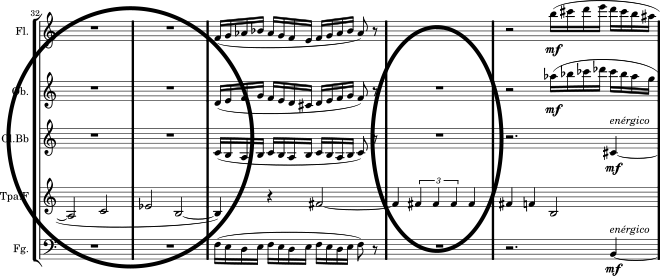
\includegraphics[scale=.7]{a-preenchimento}
    \label{fig:preenchimento-antes}
  }

  \subfloat[Preenchido depois]{
    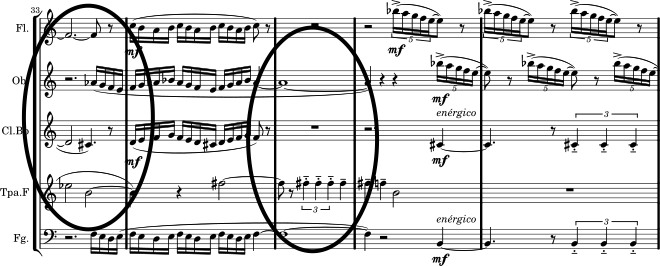
\includegraphics[scale=.7]{b-preenchimento}
    \label{fig:preenchimento-depois}
  }
  \caption{Preenchimento de vazio orquestral}
  \label{fig:preenchimento-vazio-orquestral}
\end{figure*}

O material de semicolcheias usado nos primeiros 27 compassos da peça
ficava desgastado e repetitivo ao ser reaproveitado nos compassos 30 a
45 (fig.~\ref{fig:material-esgotado-antes}). A solução encontrada foi
substituir o material original pelo fragmento em quintinas do final da
obra (fig.~\ref{fig:material-esgotado-depois}).

\begin{figure*}
  \centering
  \subfloat[Repetição antes]{
    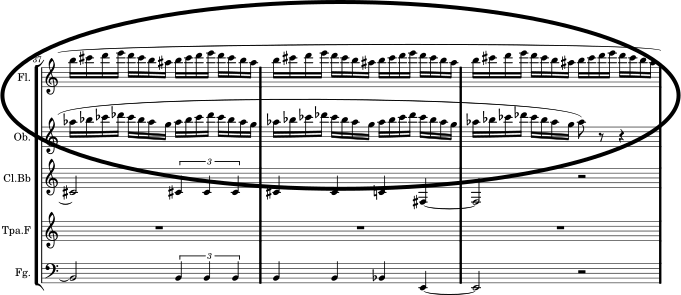
\includegraphics[scale=.7]{a-material-esgotado}
    \label{fig:material-esgotado-antes}
  }

  \subfloat[Novo material depois]{
    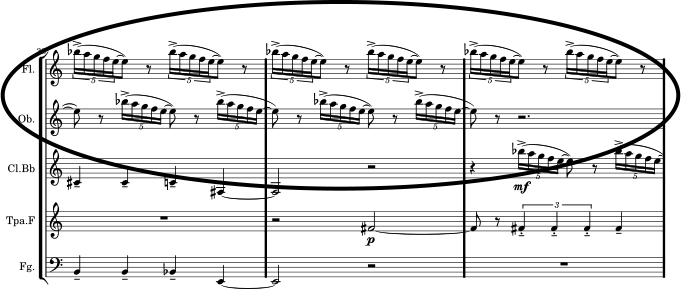
\includegraphics[scale=.7]{b-material-esgotado}
    \label{fig:material-esgotado-depois}
  }
  \caption{Reposição de material esgotado}
  \label{fig:reposicao-material-esgotado}
\end{figure*}

Seções de solo não tinham personalidade por causa de notas muito
longas não articuladas. A solução escolhida foi figurar estas notas
longas e melhorar incluir uma articulação mais precisa. Por exemplo, a
figura~\ref{fig:figuracao-antes} contém um solo para flauta (indicado
pelo número 1) com notas longas não articuladas. O mesmo solo ganhou
uma versão figurada e articulada na nova versão
(fig.~\ref{fig:figuracao-depois}).

Alguns pontos continham fragilidades referentes a vazios orquestrais e
desenho gestual. Estes trechos foram estreitados. Por exemplo, a
figura~\ref{fig:figuracao-antes} contém um trecho com essa fragilidade
(indicado pelos números 2 e 5). A distância entre as entradas dos
instrumentos foi reduzida, solucionando os problemas
(fig.~\ref{fig:figuracao-depois}).

\begin{figure*}
  \centering
  \subfloat[Antes]{
    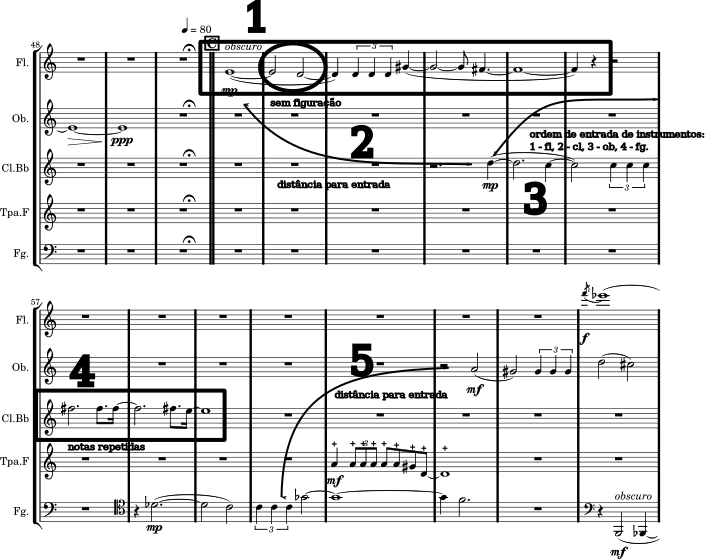
\includegraphics[scale=.7]{a-figuracao}
    \label{fig:figuracao-antes}
  }

  \subfloat[Depois]{
    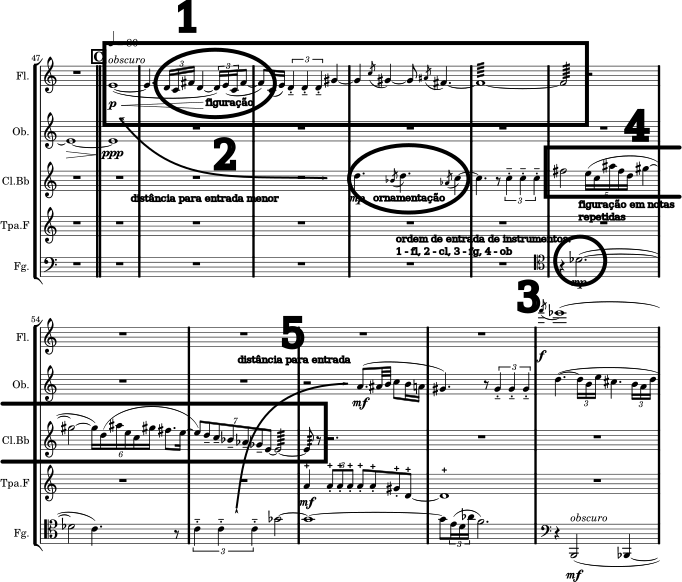
\includegraphics[scale=.7]{b-figuracao}
    \label{fig:figuracao-depois}
  }
  \caption{Melhorias diversas}
  \label{fig:figuracao}
\end{figure*}

Um dos principais materiais da peça contém notas repetidas (vide solo
da flauta da figura~\ref{fig:regularidade-antes}). Na versão anterior
essas notas não estavam bem articuladas, com pouca precisão na
escrita. Esta falta de precisão influenciava toda a peça. A solução
encontrada foi inserir uma pausa após a primeira nota, e aumentar a
precisão na escrita das articulações
(fig.~\ref{fig:regularidade-depois}).

Este problema de notas repetidas, em outros trechos, foi resolvido com
uma maior figuração rítmica. Um exemplo desta solução é ilustrada com
as figuras~\ref{fig:figuracao-antes} e~\ref{fig:figuracao-depois},
número 4.

Finalmente, um problema identificado, de alta previsibilidade por
causa da regularidade rítmica (fig.~\ref{fig:regularidade-antes}) foi
solucionado por meio de ligeiras antecipações e retardos rítmicos de
entradas de notas (fig.~\ref{fig:regularidade-depois}).

\begin{figure*}
  \centering
  \subfloat[Previsível e sem personalidade antes]{
    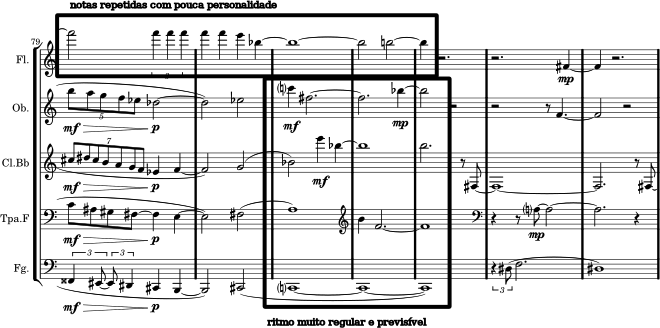
\includegraphics[scale=.7]{a-regularidade}
    \label{fig:regularidade-antes}
  }

  \subfloat[Articulado e com ritmo menos regular depois]{
    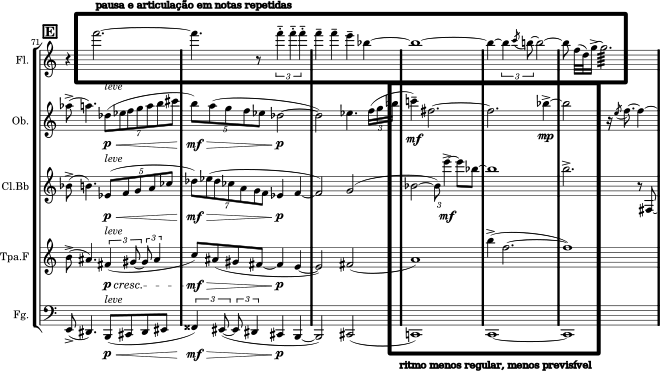
\includegraphics[scale=.7]{b-regularidade}
    \label{fig:regularidade-depois}
  }
  \caption{Repetição de notas e regularidade rítmica}
  \label{fig:regularidade}
\end{figure*}

\section{Resultado}
\label{sec:resultado}

O principal resultado da disciplina foi a nova edição da obra, com
melhorias significativas do seu aspecto composicional. As duas versões
da partitura, a de 2007 e a resultante deste trabalho estão em anexo e
podem ser comparadas.

\section{Conclusão}
\label{sec:conclusao}

Com este trabalho pude elevar a qualidade musical de uma peça antiga
interessante, com boa construção formal, bons materiais e boas
soluções composicionais, mas com trechos frágeis. Este trabalho criou
o estímulo para, futuramente, revisar outras obras antigas, tanto para
elevar a qualidade musical, quanto para servir como fonte de materiais
para novas composições.

\end{document}